\problemname{\problemyamlname}

\begin{wrapfigure}{r}{5.5cm}
    \centering
    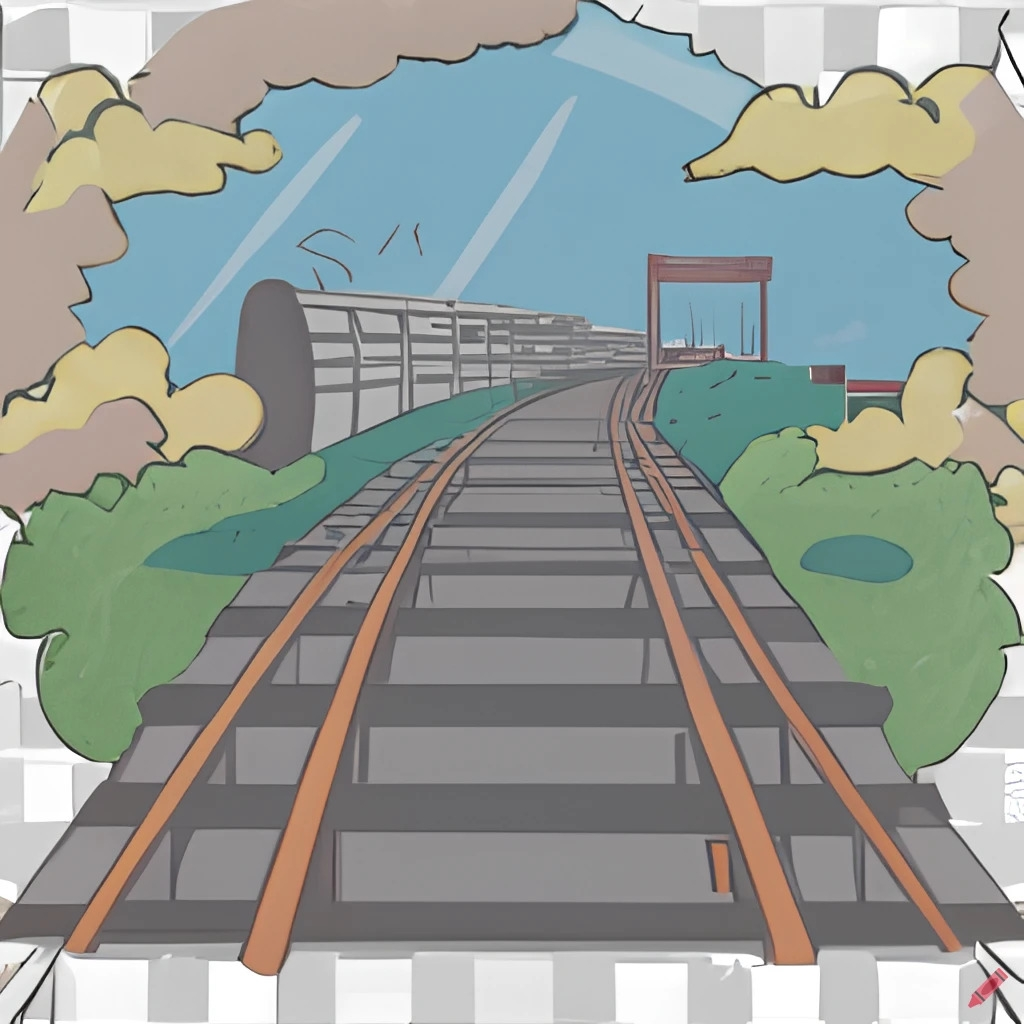
\includegraphics[width=5.5cm]{railway.jpg}
\end{wrapfigure}
Dans le cadre de la compagne \emph{Circuit Confort}, Bertrand Karwa et son équipe de Sécurail sont réhabilités
temporairement pour gérer la sécurité de plusieurs lignes ferroviaires belges. Ils reçoivent une liste de lignes
entre deux gares à emprunter, et ils doivent passer au moins une fois sur chaque ligne afin de montrer aux
voyageurs que ``le vol, ce n'est pas typique de la Belgique'' et ainsi les rassurer.

Ils souhaitent optimiser leur chemin afin d'emprunter chaque ligne de train exactement une fois, indépendamment du sens dans lequel il la prenne, mais ils ne sont pas sûrs
de la faisabilité de la tâche. Aidez-les à déterminer s'il leur est possible \textbf{en démarrant à une gare donnée}, de suivre un chemin pour \textbf{rentrer à cette même gare} et en passant \textbf{une et une seule fois} sur chaque ligne de train.

\begin{Input}
    L'entrée consiste en :
    \begin{itemize}
        \item une ligne avec un entier $n$ ($3 \le n \le 10^3$), le nombre de lignes de chemin de fer que Mr. Karwa et son équipe doivent emprunter,
        \item une ligne avec un nom de gare, là d'où doivent partir Mr. Karwa et son équipe,
        \item $n$ lignes contenant un chemin à emprunter entre deux gares, c'est-à-dire deux chaînes de caractères séparées par un espace ``\verb|gare1 gare2|'' pour dire qu'ils doivent emprunter soit la ligne de ``\verb|gare1|'' à ``\verb|gare2|'' ou soit de ``\verb|gare2|'' à ``\verb|gare1|'' (mais pas les deux).
    \end{itemize}
    Les noms de gares sont donnés en lettres alphabétiques minuscules.
    Une ligne de train entre deux gares ne sera donnée qu'une seule fois et agit comme une ligne à double sens.
\end{Input}

\begin{Output}
    S'il est impossible pour Mr. Karwa et son équipe de visiter exactement une fois chaque ligne de train donnée, donnez en sortie ``\verb|impossible|'', sinon donnez ``\verb|ok|''.
\end{Output}
